%%%%%%%%%%%%%%%%%%%%%%%%%%%%%%%%%%%%%%%%%
% University/School Laboratory Report
% LaTeX Template
% Version 3.1 (25/3/14)
%
% This template has been downloaded from:
% http://www.LaTeXTemplates.com
%
% Original author:
% Linux and Unix Users Group at Virginia Tech Wiki 
% (https://vtluug.org/wiki/Example_LaTeX_chem_lab_report)
%
% License:
% CC BY-NC-SA 3.0 (http://creativecommons.org/licenses/by-nc-sa/3.0/)
%
%%%%%%%%%%%%%%%%%%%%%%%%%%%%%%%%%%%%%%%%%

%----------------------------------------------------------------------------------------
%	PACKAGES AND DOCUMENT CONFIGURATIONS
%----------------------------------------------------------------------------------------

\documentclass{article}

\usepackage[version=3]{mhchem} % Package for chemical equation typesetting
\usepackage{siunitx} % Provides the \SI{}{} and \si{} command for typesetting SI units
\usepackage{graphicx} % Required for the inclusion of images
\usepackage{natbib} % Required to change bibliography style to APA
\usepackage{amsmath} % Required for some math elements
\usepackage{tcolorbox} % Provide a frame around text
\usepackage{tabto}
\usepackage[normalem]{ulem}

\setlength\parindent{0pt} % Removes all indentation from paragraphs

\renewcommand{\labelenumi}{\alph{enumi}.} % Make numbering in the enumerate environment by letter rather than number (e.g. section 6)

%\usepackage{times} % Uncomment to use the Times New Roman font

%----------------------------------------------------------------------------------------
%	DOCUMENT INFORMATION
%----------------------------------------------------------------------------------------

\title{HADOOP \\ TP MapReduce} % Title

\author{Nicolas \textsc{Lagaillardie}} % Author name

\date{\today} % Date for the report

\begin{document}

\maketitle % Insert the title, author and date

%\begin{center}
%\begin{tabular}{l r}
%Date Performed: & January 1, 2012 \\ % Date the experiment was performed
%Partners: & James Smith \\ % Partner names
%& Mary Smith \\
%Instructor: & Professor Smith % Instructor/supervisor
%\end{tabular}
%\end{center}

% If you wish to include an abstract, uncomment the lines below
% \begin{abstract}
% Abstract text
% \end{abstract}

%----------------------------------------------------------------------------------------
%	SECTION 1
%----------------------------------------------------------------------------------------

\section{Objectif}

Exp\'{e}rimenter le fonctionnement d'Hadoop \`{a} travers un exemple : calcul de la fr\'{e}quence des mots pr\'{e}sents dans les ouvrages de l'ABU puis calcule l’index des mots pr\'{e}sents dans les ouvrages de l’ABU.

%\begin{center}\ce{2 Mg + O2 - 2 MgO}\end{center}

% If you have more than one objective, uncomment the below:
%\begin{description}
%\item[First Objective] \hfill \\
%Objective 1 text
%\item[Second Objective] \hfill \\
%Objective 2 text
%\end{description}

\subsection{D\'{e}finitions}
\label{definitions}
\begin{description}
\item[Hadoop]
Un logiciel open-source pour r\'{e}aliser des op\'{e}rations informatiques des mani\`{e}re fiable, \'{e}volutif et distribu\'{e}e.
\item[Pseudo-distributed mode]
Un mode qui permet d'\'{e}muler le fonctionnement d'op\'{e}rations distribu\'{e}es sur plusieurs machines sur une m\^{e}me machine. On parle alors de pseudo-cluster.
\end{description} 
 
%----------------------------------------------------------------------------------------
%	SECTION 2
%----------------------------------------------------------------------------------------

\section{Donn\'{e}es exp\'{e}rimentales}

\begin{description}
\item[ABU]
Un ensemble de 202 fichiers txt, provenant d'\oe uvres fran\c{c}aises. Les mots poss\`{e}dent donc des accents et d'autres caract\`{e}res, \`{a} prendre en consid\'{e}ration dans le d\'{e}compte.
\end{description} 

%----------------------------------------------------------------------------------------
%	SECTION 3
%----------------------------------------------------------------------------------------

\section{Pr\'{e}requis}

L'ensemble des \'{e}tapes sont d\'{e}taill\'{e}es sur le site internet d'Hadoop. Il s'agit d'abord d'avoir les logiciels pr\'{e}requis : \textbf{ssh}, \textbf{rysinc} et \textbf{Java}. Puis il faut assigner \`{a} Hadoop le chemin vers \textbf{Java}. En effet, Hadoop utilise Java pour fonctionner. Pour ma part, il a \'{e}t\'{e} n\'{e}cessaire que j'utilise \textbf{JDK} et non \textbf{JSE}, car certaines classes manquaient \`{a} l'appel. Nous sommes ensuite pr\^{e}ts \`{a} lancer le \textbf{pseudo-cluster}.

%----------------------------------------------------------------------------------------
%	SECTION 4
%----------------------------------------------------------------------------------------

\section{Installation du pseudo-cluster}

Comme nous n'avons pas imm\'{e}diatement acc\`{e}s \`{a} un cluster complet, nous allons lancer un pseudo-cluster. C'est-\`{a}-dire que nous allons simuler un cluster, avec un \textit{namenode} et un \textit{datanode}.

Nous devons d'abord configurer le port d'utilisation d'Hadoop puis sp\'{e}cifier le nombre de \textit{namenodes} utilis\'{e}s. Dans notre cas, voici la configuration utilis\'{e}e : \\* \\*
Modification du fichier \textit{core-site.xml} :

\begin{tcolorbox}
\textless configuration\textgreater \\*
\tabto{1cm} \textless property\textgreater \\*
\tabto{2cm} \textless name\textgreater fs.defaultFS\textless /name\textgreater \\*
\tabto{2cm} \textless value\textgreater hdfs://localhost:9000\textless /value\textgreater \\*
\tabto{1cm} \textless /property\textgreater \\*
\textless /configuration\textgreater
\end{tcolorbox}
~\\
Modification du fichier \textit{hdfs-site.xml} :

\begin{tcolorbox}
\textless configuration\textgreater \\*
\tabto{1cm} \textless property\textgreater \\*
\tabto{2cm} \textless name\textgreater dfs.replication\textless /name\textgreater \\*
\tabto{2cm} \textless value\textgreater 1\textless /value\textgreater 
\tabto{1cm} \textless /property\textgreater \\*
\textless /configuration\textgreater
\end{tcolorbox}
~\\
Il faut ensuite se connecter au \textit{ssh} pour que Hadoop puisse communiquer avec ses autres pseudo \textit{datanodes}.

\begin{tcolorbox}
\$ ssh localhost
\end{tcolorbox}

%\begin{figure}[h]
%\begin{center}
%
\includegraphics[width=0.65\textwidth]{placeholder} % Include the image placeholder.png
%\caption{Figure caption.}
%\end{center}
%\end{figure}

%----------------------------------------------------------------------------------------
%	SECTION 5
%----------------------------------------------------------------------------------------

\section{Ex\'{e}cution du \textit{MapReduce}}

Nous allons maintenant lancer notre script afin de pouvoir d\'{e}compter le nombre de mots dans l'ensemble des fichiers txt. Il faut 6 \'{e}tapes pour y arriver.

\begin{enumerate}
\begin{item}
Formatage de l'espace de stockage
\begin{tcolorbox}
\$ bin/hdfs namenode -format
\end{tcolorbox}
\end{item}
\begin{item}
D\'{e}marrage du \textit{namenode} et du \textit{datanode}
\begin{tcolorbox}
\$ sbin/start-dfs.sh
\end{tcolorbox}
\end{item}
\begin{item}
Cr\'{e}ation des dossiers \textit{user} sur le cluster
\begin{tcolorbox}
\$ bin/hdfs dfs -mkdir /user
\$ bin/hdfs dfs -mkdir /user/Lag
\end{tcolorbox}
\end{item}
\begin{item}
Ajout des fichiers dans le cluster
\begin{tcolorbox}
\$ bin/hdfs dfs -put ABU /user/Lag
\end{tcolorbox}

\begin{figure}[h]
\begin{center}
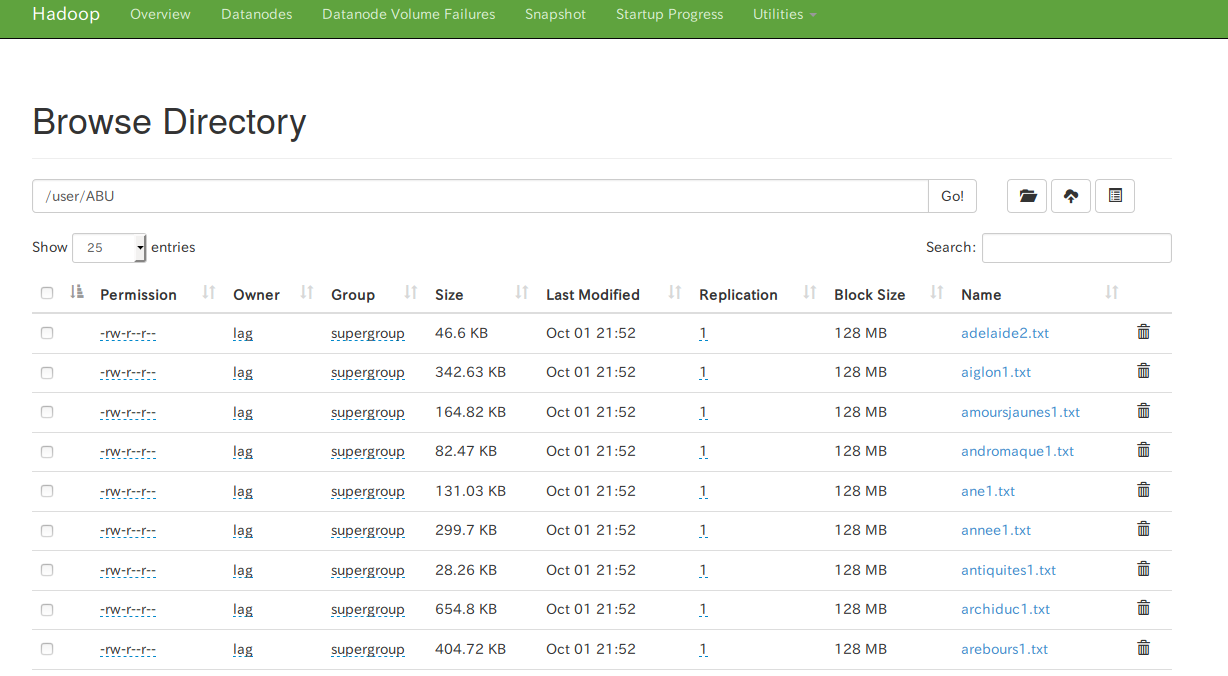
\includegraphics[width=0.85\textwidth]{insideDatanode}
\caption{Contenu du cluster}
\label{fig:datanodeContent}
\end{center}
\end{figure}

\end{item}
\begin{item}
Compiler puis ex\'{e}cuter notre script java
\begin{tcolorbox}
\$ bin/hadoop com.sun.tools.javac.Main WordCount.java \\*
\$ jar cf WC.jar WordCount*.class \\*
\$ bin/hadoop jar WC.jar WordCount /user/Lag/ABU /user/output
\end{tcolorbox}
\end{item}
\begin{item}
R\'{e}cup\'{e}rer puis afficher les r\'{e}sultats
\begin{tcolorbox}
\$ bin/hdfs dfs -ls /user/output \\*
\$ bin/hdfs dfs -cat '/user/output/part-*'
\end{tcolorbox}
\end{item}
\end{enumerate}

%----------------------------------------------------------------------------------------
%	SECTION 6
%----------------------------------------------------------------------------------------

\section{Premiers r\'{e}sultats}

Suite au lancement de la premi\`{e}re version du script, voici les r\'{e}sultats : ils sont globalement satisfaisants (voir Figure \ref{fig:firstResultsErrorLess}, mais de nombreux probl\`{e}mes persistents (voir Figure ~\ref{fig:firstResultsError}).

\begin{figure}[h]
\begin{center}
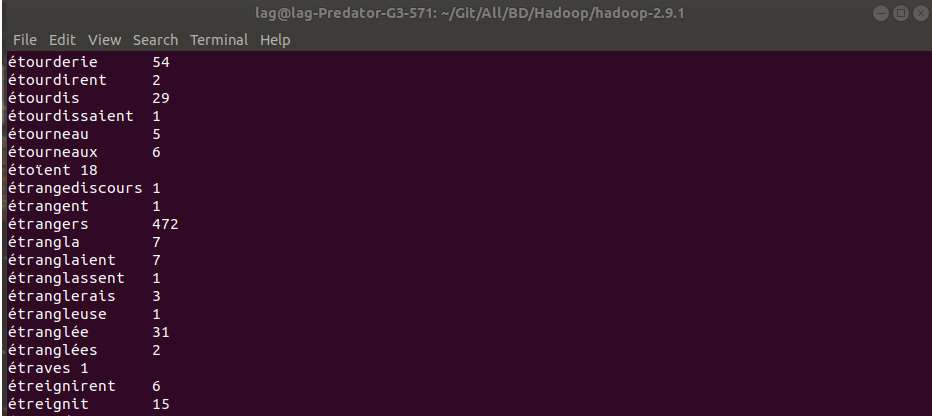
\includegraphics[width=0.85\textwidth]{console_resultat_2}
\caption{premiers r\'{e}sultats}
\label{fig:firstResultsErrorLess}
\end{center}
\end{figure}

\begin{figure}[h]
\begin{center}
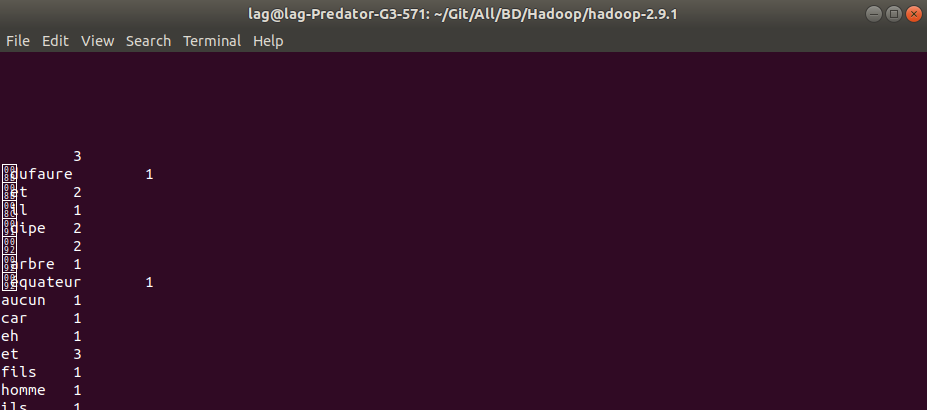
\includegraphics[width=0.85\textwidth]{console_resultat_erreur}
\caption{premi\`{e}res erreurs}
\label{fig:firstResultsError}
\end{center}
\end{figure}

Dans cette deuxi\`{e}me capture d'\'{e}cran, nous remarquons que certains caract\`{e}res accentu\'{e}s sont mal repr\'{e}sent\'{e}s. Tandis que d'autres caract\`{e}res que nous n'avons pas d\^{u} prendre en compte dans notre script pour s\'{e}parer les mots cr\'{e}ent des erreurs non voulues. \\*

%----------------------------------------------------------------------------------------
%	SECTION 7
%----------------------------------------------------------------------------------------

\section{Correction et second r\'{e}sultats}

Les modifications possibles concernent la s\'{e}paration et le comptage des motss des diff\'{e}rents fichiers. \\*
Voici une nouvelle s\'{e}paration possible, qui ne d\'{e}pend pas de caract\`{e}res que nous \'{e}tablissons nous-m\^{e}me, mais de l'impl\'{e}mentation m\^{e}me de l'encodage. Ainsi, le code suivant : \\*

\begin{tcolorbox}
StringTokenizer itr = new StringTokenizer( \\*
\tabto{1cm} value.toString().toLowerCase(), \\*
\tabto{1cm} " \textbackslash t\textbackslash n\textbackslash r\textbackslash f.,;:-'\textbackslash "\textbackslash \textbackslash ()!?/{[}]«»\# =/+`* \$ 0123456789” \\*
); \\*
while (itr.hasMoreTokens()) \{ \\*
\tabto{1cm} word.set(itr.nextToken()); \\*
\tabto{1cm} context.write(word, one); \\*
); \\*
\end{tcolorbox}
~ \\*
Est remplac\'{e} par celui-ci :

\begin{tcolorbox}
FileSplit fileSplit = (FileSplit)context.getInputSplit(); \\*
String filename = fileSplit.getPath().getName(); \\*
Path filePath = fileSplit.getPath(); \\*
String fileName = filePath.getName(); \\*

valueOutFilename = new Text(fileName); \\*

for (String word : StringUtils.split(valueIn.toString())) \{ \\*
\tabto{1cm} context.write(new Text(word), valueOutFilename); \\*
\}
\end{tcolorbox}
~ \\*

Nous avons ainsi une s\'{e}paration mieux d\'{e}finie et une concat\'{e}nation de tous les r\'{e}sultats, au lieu de plusieurs fichiers r\'{e}sultats avec peu de coh\'{e}rence entre chacun d'eux.

La deuxi\`{e}me partie a consist\'{e} \`{a} modifier le \textit{Reducer} afin qu'il comptabilise les fichiers contenant les mots et non le nombre d'occurences de ces derniers. Voici le code que nous avons modifi\'{e} : \\*

\begin{tcolorbox}
private IntWritable result = new IntWritable (); \\*
	
int sum = 0; \\*

for (IntWritable val : values) \{ \\*
\tabto{1cm} sum += val.get(); \\*
\} \\*

result.set(sum); \\*
context.write(key, result);
\end{tcolorbox}
~ \\*
En ce code :

\begin{tcolorbox}
HashSet\textless String\textgreater  fileNamesUnique = new HashSet\textless String\textgreater (); \\*

for (Text fileName: valuesInFileNames) \{ \\*
\tabto{1cm} fileNamesUnique.add(fileName.toString()); \\*
\} \\*

String fileNamesOut = new String( StringUtils.join(fileNamesUnique, " / ") ); \\*

context.write(keyInWord, new Text(fileNamesOut));
\end{tcolorbox}
~ \\*

Remarquons que j'ai choisi d'utiliser la fonction de hashage pr\'{e}sente dans Java, afin d'acc\'{e}l\'{e}rer le traitement des donn\'{e}es. Nous pouvons observer les r\'{e}sultats de l'ex\'{e}cution dans la figure \ref{fig:goodResults} o\`{u} nous pouvons constater que pour chaque mot, les fichiers le contenant sont affich\'{e}s \`{a} la suite.

\begin{figure}[h]
\begin{center}
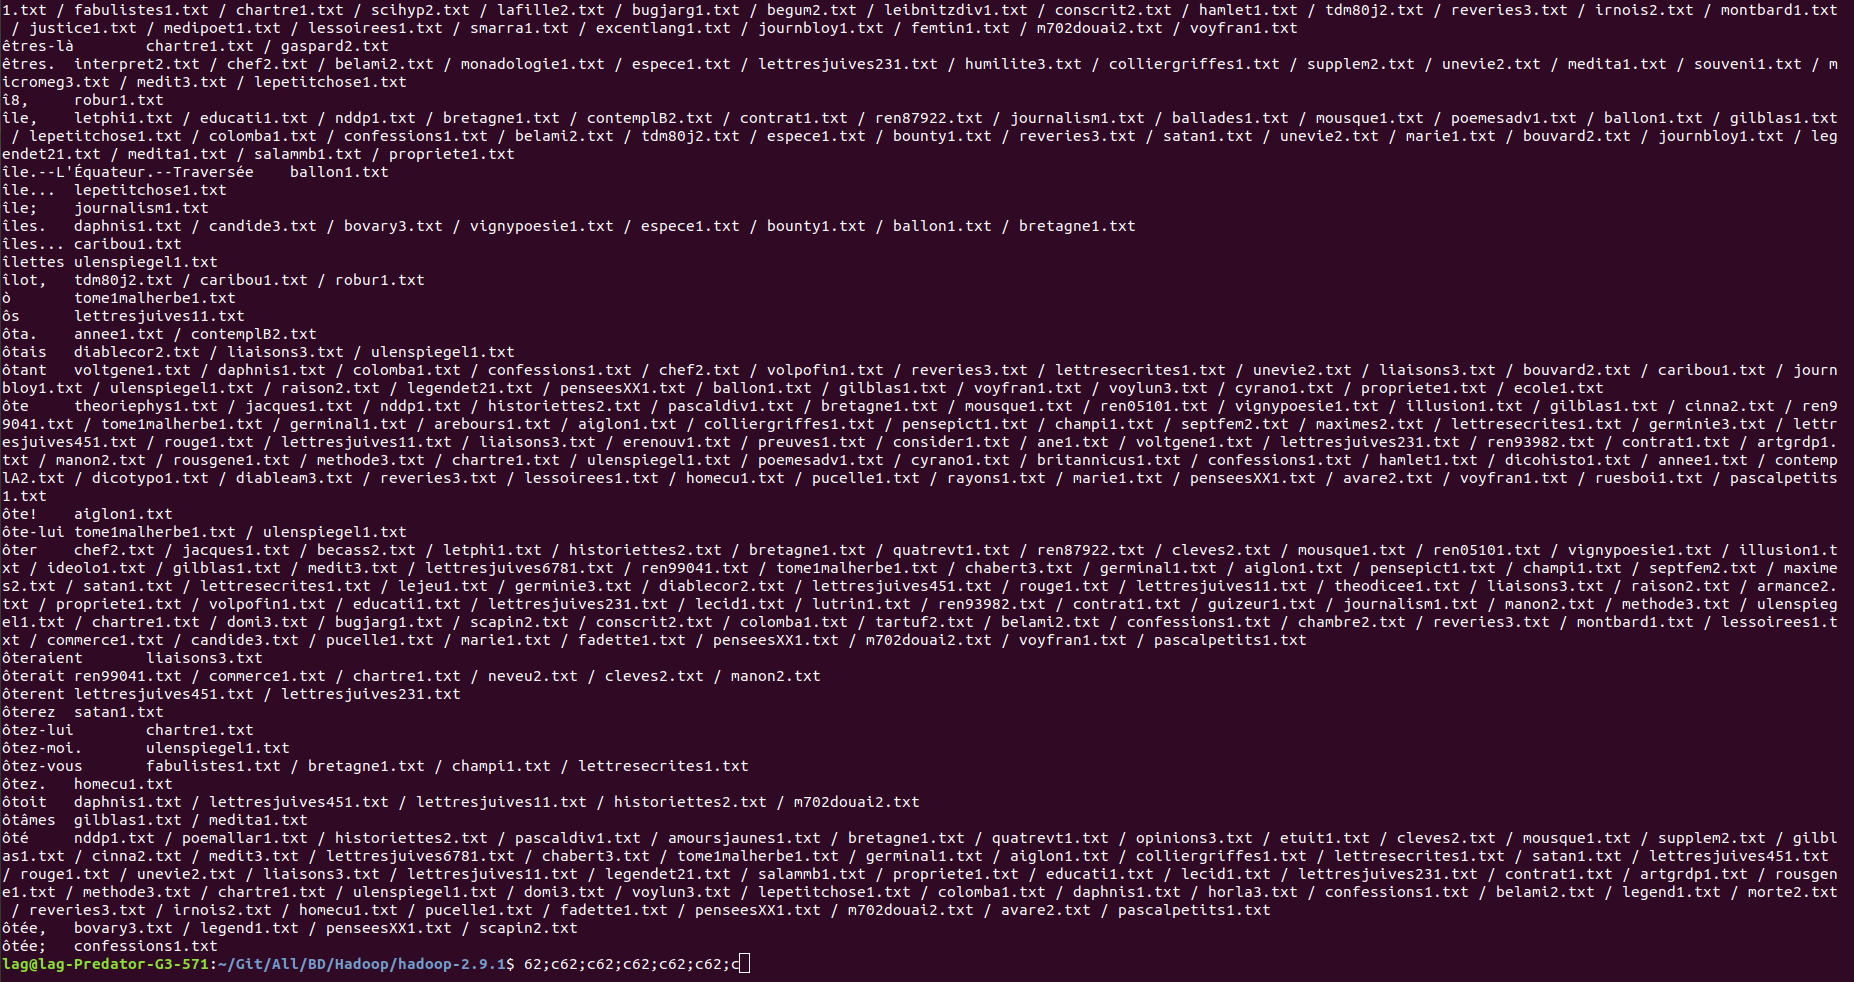
\includegraphics[width=1\textwidth]{GoodResults}
\caption{Index des mots}
\label{fig:goodResults}
\end{center}
\end{figure}

\pagebreak

%----------------------------------------------------------------------------------------
%	SECTION 8
%----------------------------------------------------------------------------------------

\section{Conclusion}

Hadoop est un puissant syst\`{e}me et ce TP a pu d\'{e}montrer une des utilisations possibles. A l'aide d'un \textit{simple} script Java, nous avons \'{e}t\'{e} en mesure de cr\'{e}er un index des mots pr\'{e}sents dans 202 fichiers txt. Nous avons pu aussi utiliser un compteur de mots performant mais l\'{e}g\`{e}rement d\'{e}faillant, que nous avons corrig\'{e} par la suite. \\*
Par ailleurs, l'installation et l'utilisation d'Hadoop est bien document\'{e}e et assez simple  en mode Pseudo-cluster.

%----------------------------------------------------------------------------------------
%	BIBLIOGRAPHY
%----------------------------------------------------------------------------------------

%\bibliographystyle{apalike}
%
%\bibliography{sample}

%----------------------------------------------------------------------------------------


\end{document}